\documentclass[12pt,oneside]{book} % for one-sided printing

\usepackage{blindtext}% Just used so we can generate some example text
\usepackage{amsmath}
\usepackage{amssymb}
\usepackage{mathtools}
\usepackage[export]{adjustbox}
\usepackage{lipsum}
\usepackage{booktabs}  % For better quality tables
\usepackage{tabularx}  % for the X column type
\usepackage{listings}
\usepackage{xcolor}
\usepackage{caption}
\usepackage{xfrac}
\usepackage{algorithmic}
\usepackage{indentfirst}
\usepackage{subcaption}
\usepackage{graphicx}
\usepackage{geometry}
\geometry{a4paper, margin=1in}

% Place style file after other packages.
\usepackage{cranfieldthesis}
\usepackage{lscape} % for landscape pages
\usepackage{float}
\usepackage[toc,title,page]{appendix}

% Couleurs personnalisées
\definecolor{backcolour}{rgb}{0.96, 0.96, 0.96} % Fond très clair
\definecolor{codegray}{rgb}{0.47, 0.47, 0.47}   % Commentaires et numéros de ligne
\definecolor{codegreen}{rgb}{0.25, 0.50, 0.35}  % Commentaires
\definecolor{codeblue}{rgb}{0.26, 0.44, 0.58}   % Mots-clés
\definecolor{codepurple}{rgb}{0.50, 0, 0.50}    % Identificateurs
\definecolor{codeteal}{rgb}{0, 0.5, 0.5}        % Chaînes de caractères
\definecolor{terminalback}{rgb}{0.05, 0.05, 0.05} % Fond très sombre pour le terminal
\definecolor{terminaltext}{rgb}{0.7, 0.7, 0.7}    % Texte clair pour le terminal

\lstdefinestyle{python}{
    language=Python,
    backgroundcolor=\color{backcolour},
    commentstyle=\color{codegreen},
    keywordstyle=\color{codeblue},
    numberstyle=\tiny\color{codegray},
    stringstyle=\color{codeteal},
    identifierstyle=\color{codepurple},
    basicstyle=\ttfamily\scriptsize,
    breakatwhitespace=false,
    breaklines=true,
    captionpos=b,
    keepspaces=true,
    numbers=left,
    numbersep=5pt,
    showspaces=false,
    showstringspaces=false,
    showtabs=false,
    tabsize=4,
    frame=single,
    rulecolor=\color{codegray},
    framexleftmargin=15pt,
    framextopmargin=5pt,
    framexbottommargin=5pt,
    framexrightmargin=15pt,
}

\lstdefinestyle{terminal}{
    backgroundcolor=\color{terminalback}, % Background color
    basicstyle=\color{terminaltext}\ttfamily\scriptsize, % Text style
    frame=single, % Frame style
    rulecolor=\color{codegray}, % Frame color
    framexleftmargin=15pt, % Left margin
    framextopmargin=5pt, % Top margin
    framexbottommargin=5pt, % Bottom margin
    framexrightmargin=15pt, % Right margin
    breaklines=true, % Automatic line breaking
    captionpos=b, % Caption position (bottom in this case)
    keepspaces=true, % Keep spaces for indentation
    showspaces=false, % Do not show spaces explicitly
    showstringspaces=false, % Do not show spaces in strings
    showtabs=false, % Do not show tabs
    tabsize=4, % Tab size
    numbers=none, % Line numbers (none in this case)
}

% Title Page Set Up
\title{Cloud Computing Assignment}
\author{Alexis Balayre}
\date{2\textsuperscript{nd} January 2024}
\school{\SATM}
\degree{MSc}
\course{Computational Software of Techniques Engineering}
\academicyear{2023 - 2024}

% Supervisors
\supervisor{Dr Stuart Barnes}

% Copyright
\copyrightyear{2024}

% References
\usepackage[numbers]{natbib} % for nice referencing
\makeatletter % Reference list option change to number and period
\renewcommand\@biblabel[1]{#1.} % from [1] to 1
\makeatother %
\setcitestyle{round} % use round citations

\begin{document}

\frontmatter

% Form Title Pages
\maketitle

% Use single spacing for Table of Contents, List of Figures, etc
{
    \clearpage
    \singlespacing
    % Table of Contents
    {
        \tableofcontents
    }
    \clearpage

    % List of Figures
    \listoffigures

    % List of Tables
    \listoftables
}

%% Main Matter
\mainmatter
\pagestyle{fancy}
\fancyhead[L]{\nouppercase{\leftmark}}
\fancyhead[R]{\nouppercase{\rightmark}}

\chapter{Introduction}
In an increasingly connected world, cloud computing and the Internet of Things
(IoT) are revolutionising many fields, including environmental monitoring. This
technological development offers unprecedented possibilities for managing and
analysing air quality, a major public health issue. This report, drawn up as
part of my Master's degree in Cloud and Embedded Systems Science and Technology
(CSTE), focuses on the use of these technologies to collect, process and
distribute environmental data.

The main aim of this assignment is to store and make accessible the latest air
quality data, captured by a network of small environmental IoT sensors. The
project aims to provide a reliable platform for real-time consultation of
environmental data, a crucial tool for researchers, decision-makers and the
general public.

We face a number of technical challenges in achieving this objective. Firstly,
managing the large quantities of data generated by IoT sensors requires a
robust and adaptable cloud infrastructure. Secondly, calculating the Air
Quality Index (AQI) from this data in real time requires considerable
processing power and accuracy. Finally, the need to keep the system adaptable
and responsive to varying workloads presents an additional challenge.

To address these challenges, our approach is to use a database located in the
cloud, specifically designed to manage and process large volumes of IoT data.
This database will be regularly updated with new data, while allowing quick and
easy access for end users. In addition, we will be implementing advanced
algorithms for calculating the AQI, guaranteeing the accuracy and reliability
of the information provided.

The importance of this system is not limited to environmental monitoring; it
also has a significant impact on public health, urban planning and
environmental awareness. By providing accurate and up-to-date data, we
contribute to a better understanding and management of air quality.

In conclusion, this report will detail our methodology, the architecture of the
system, the challenges encountered and the solutions adopted. We will also
discuss the implications of our work, not only in technical terms but also in
terms of its practical applications and impact on different stakeholders.

\chapter{Methodologies}\label{chap:one}

\section{Data Collecting, Processing \& Storing}

\subsection{Overview of the Pipeline Architecture}

The initial pipeline in this project consists of three primary components:
\textbf{Data Collecting}, \textbf{Data Processing}, and \textbf{Data Storing}.

During the \textbf{Data Collecting} phase, the most recent version of the
dataset is acquired from its source. This is followed by the \textbf{Data
    Processing} phase, where the data is formatted, and the Air Quality Index (AQI)
is calculated for each particulate matter sensor. Lastly, in the \textbf{Data
    Storing} phase, the data from each sensor is methodically stored in a
time-series database.

\begin{figure}[H]
    \centering
    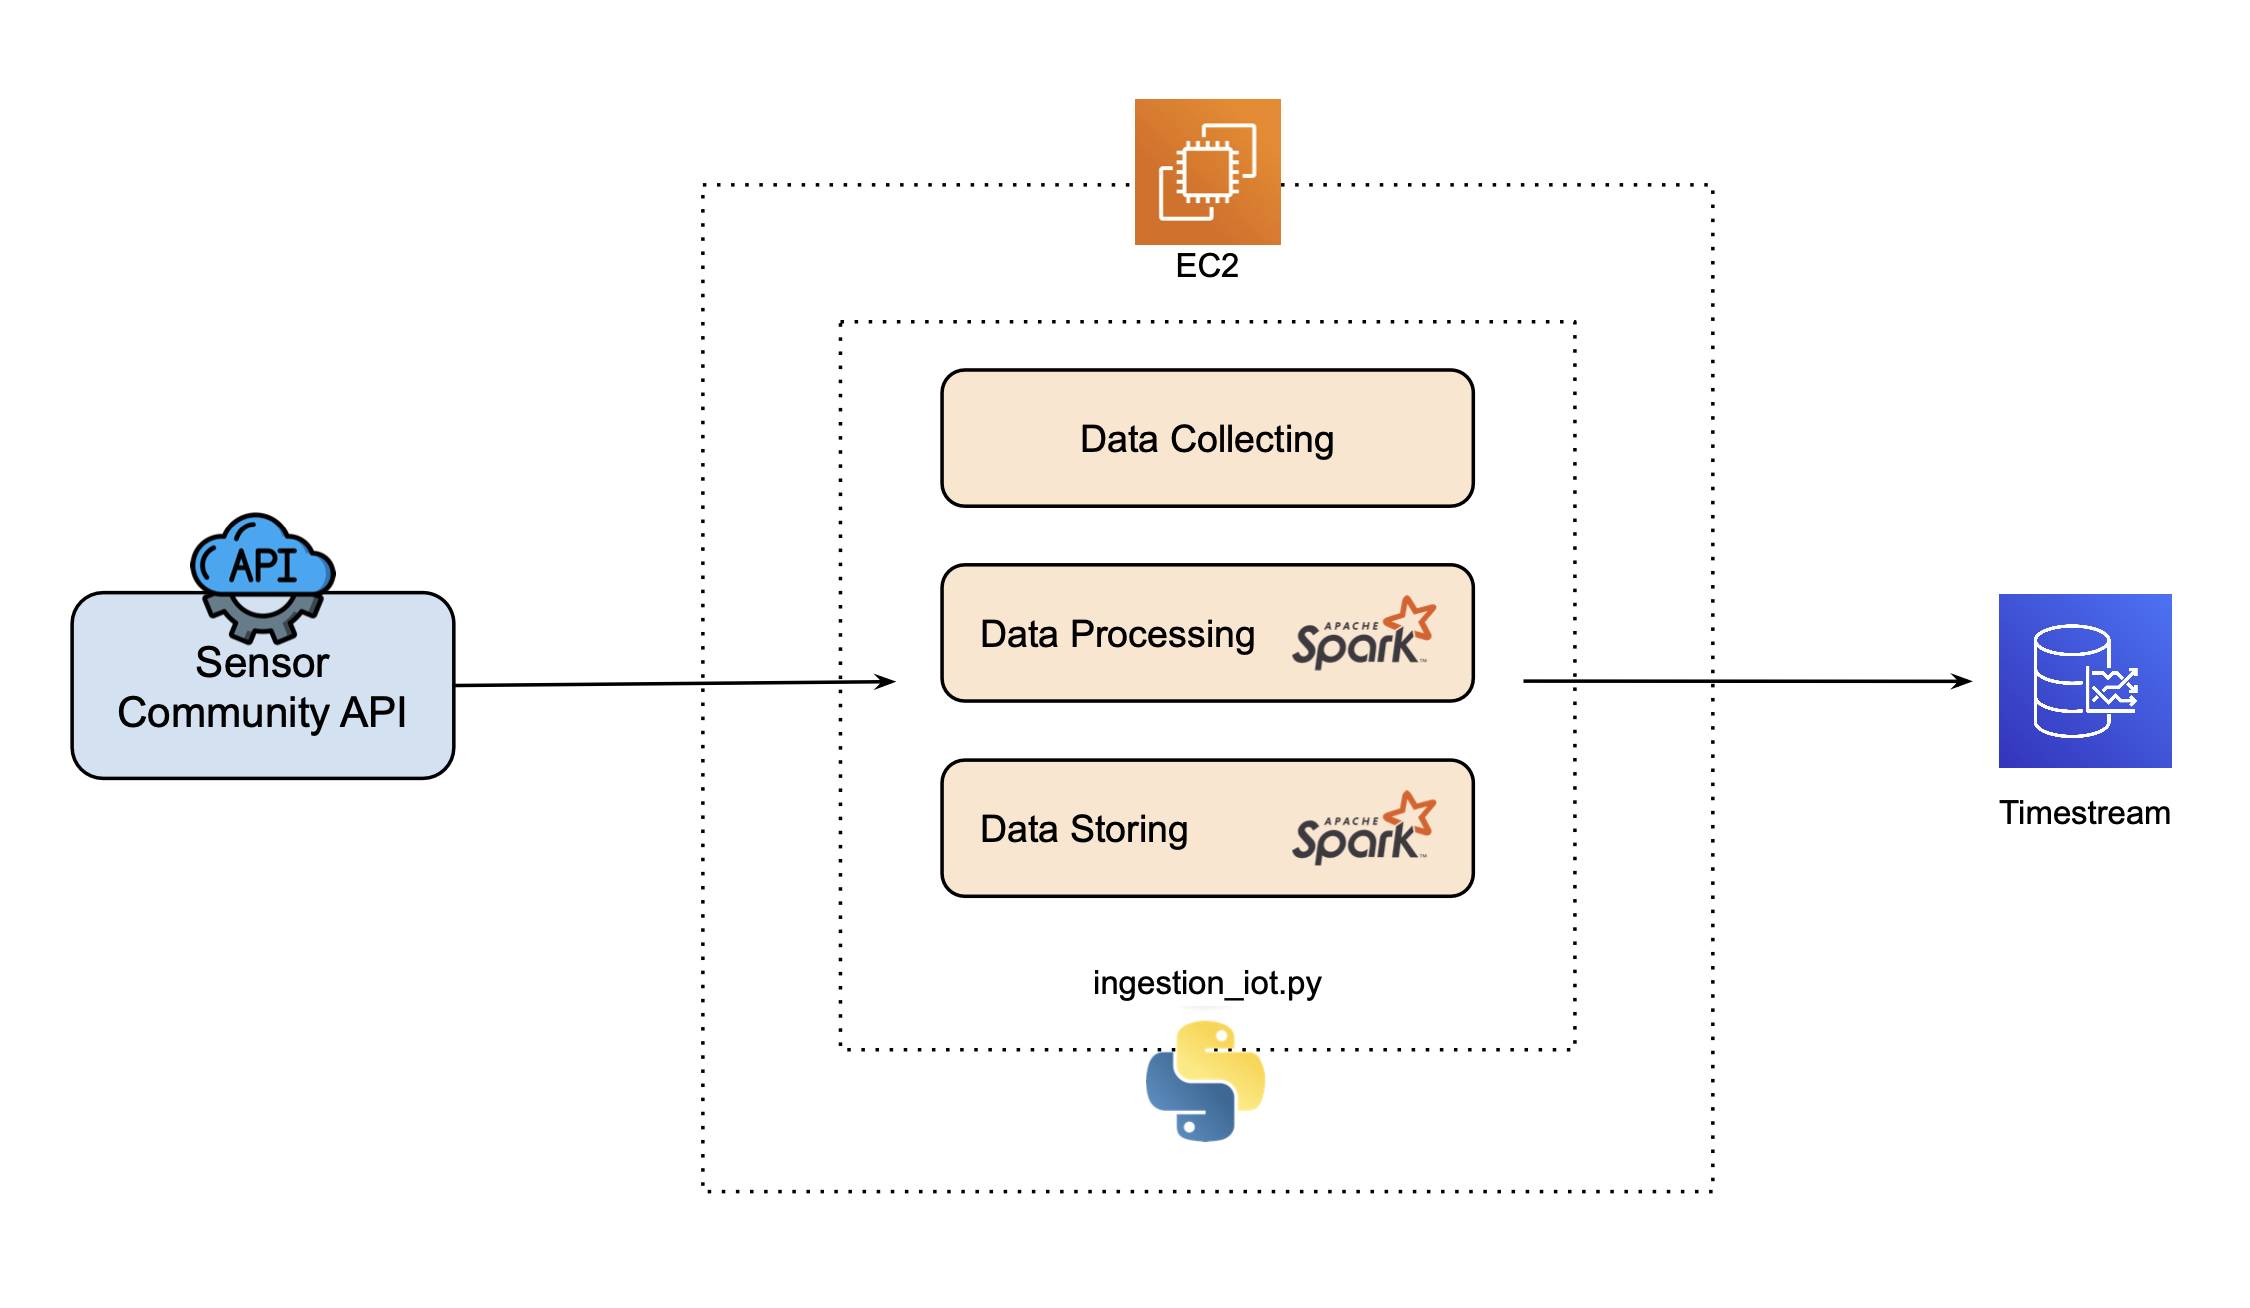
\includegraphics[width=1\linewidth]{images/cloud-computing-data-ingestion.png}
    \caption{Data Collecting, Processing \& Storing Pipeline Diagram}
\end{figure}

\subsection{Data Collecting}
\subsubsection{Data Source}
The Sensor Community network is a global, contributor-driven initiative that
collects open environmental data through a vast network of sensors. These
sensors, deployed in over 70 countries, collect real-time data on air quality,
temperature, humidity and pressure. On average, the sensors send new data every
145 seconds~\cite{sensorcommunity2023synchronization}. The Sensor Community
network offers two main API endpoints for accessing their environmental data:

\begin{enumerate}
    \item \textbf{5-Minute Averaged Data API:} This API provides data averaged over the last 5 minutes for each sensor. This is useful for near real-time analysis or immediate air quality assessments, particularly in test or active monitoring contexts.
    \item \textbf{24 Hour Averaged Data API:} This API provides data averaged over the last 24 hours for each sensor. It is particularly suited to analysing daily trends and understanding environmental changes over a longer period.
\end{enumerate}

\subsubsection{Python Script}
In this project, both APIs were used to collect data from the Sensor Community.
The data was collected using the \texttt{requests} library in Python and stored
in the cache of the local machine in a Spark DataFrame. This step is performed
every 10 seconds to ensure that the data is up to date.

\subsection{Choice of Database}
This project uses Amazon Timestream, which is a cloud-native time series
database. It is a wise choice because of its superior time series management
capabilities, which are particularly well suited to data from IoT sensors. This
database is distinguished by its speed of ingestion and efficiency in
processing vast volumes of data, facilitating regular updates and in-depth
analyses of the Air Quality Index. Its ability to adjust to variations in
workload is a major asset, ensuring consistent performance. What's more,
Timestream's advanced security features meet strict standards of
confidentiality and data sovereignty, an essential criterion for the secure
management of sensitive information.

\subsection{Query 3}

\newpage

\section{Queries Optimisation}

\newpage

\section{Pipeline of the Project}
\subsection{Pipeline Overview}

The pipeline of this project is composed of four main components: \textbf{data
    ingestion}, \textbf{query 1}, \textbf{query 2} and \textbf{query 3}.\newline

The \textbf{ingestion} task retrieves the last version of the data set from the
source and stores it in the data lake (CSV file stored in local storage). Then,
the \textbf{queries 1, 2 \& 3} tasks retrieves the data from the data lake and
performs the queries on the data.

\begin{figure}[h]
    \centering
    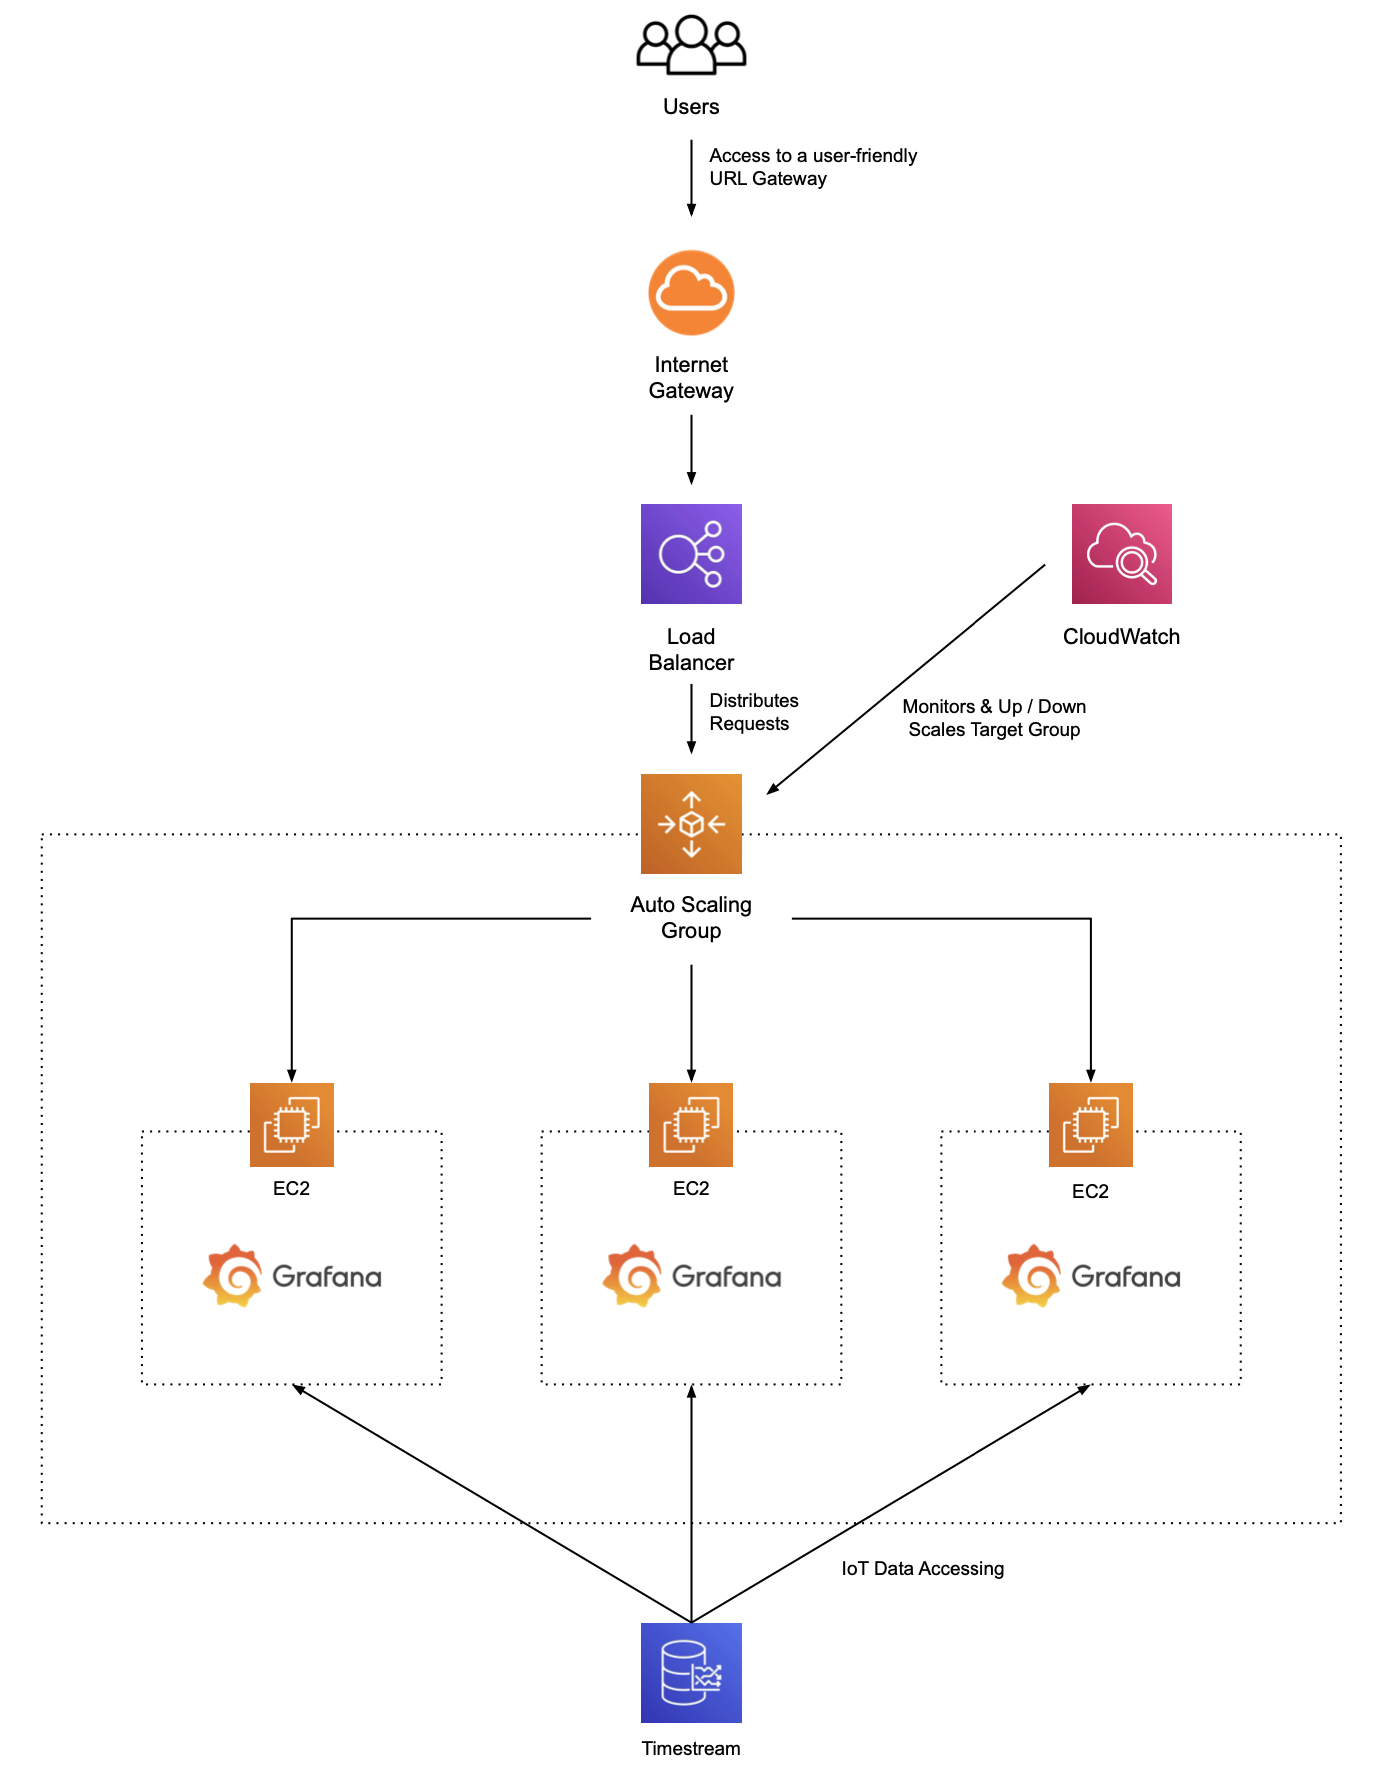
\includegraphics[width=1\linewidth]{images/cloud-computing-clients.png}
    \caption{Data Distributing Pipeline Diagram}
\end{figure}

\newpage
\subsection{Pipeline Orchestration}

In order to orchestrate and automate the pipeline, a scheduled task must be run
every day to retrieve the latest version of the dataset and run the tasks when
a new daily row is added at 23:59 UTC to the dataset.\newline

To perform this task, a DAG (Directed Acyclic Graph) was created using Apache
Airflow. The DAG is scheduled to run every day at 00:00 UTC and is composed of
four tasks: \textbf{ingestion}, \textbf{query 1}, \textbf{query 2} and
\textbf{query 3}. The screenshot below~\ref{fig:apache-airflow} shows the DAG
graph of the pipeline in the web interface of Apache Airflow.\newline

The benefits of using a workflow platform such as Apache Airflow are its
ability to schedule and automate the pipeline, as well as its ability to
monitor the pipeline and send alerts if a task fails.

\begin{figure}[h]
    \centering
    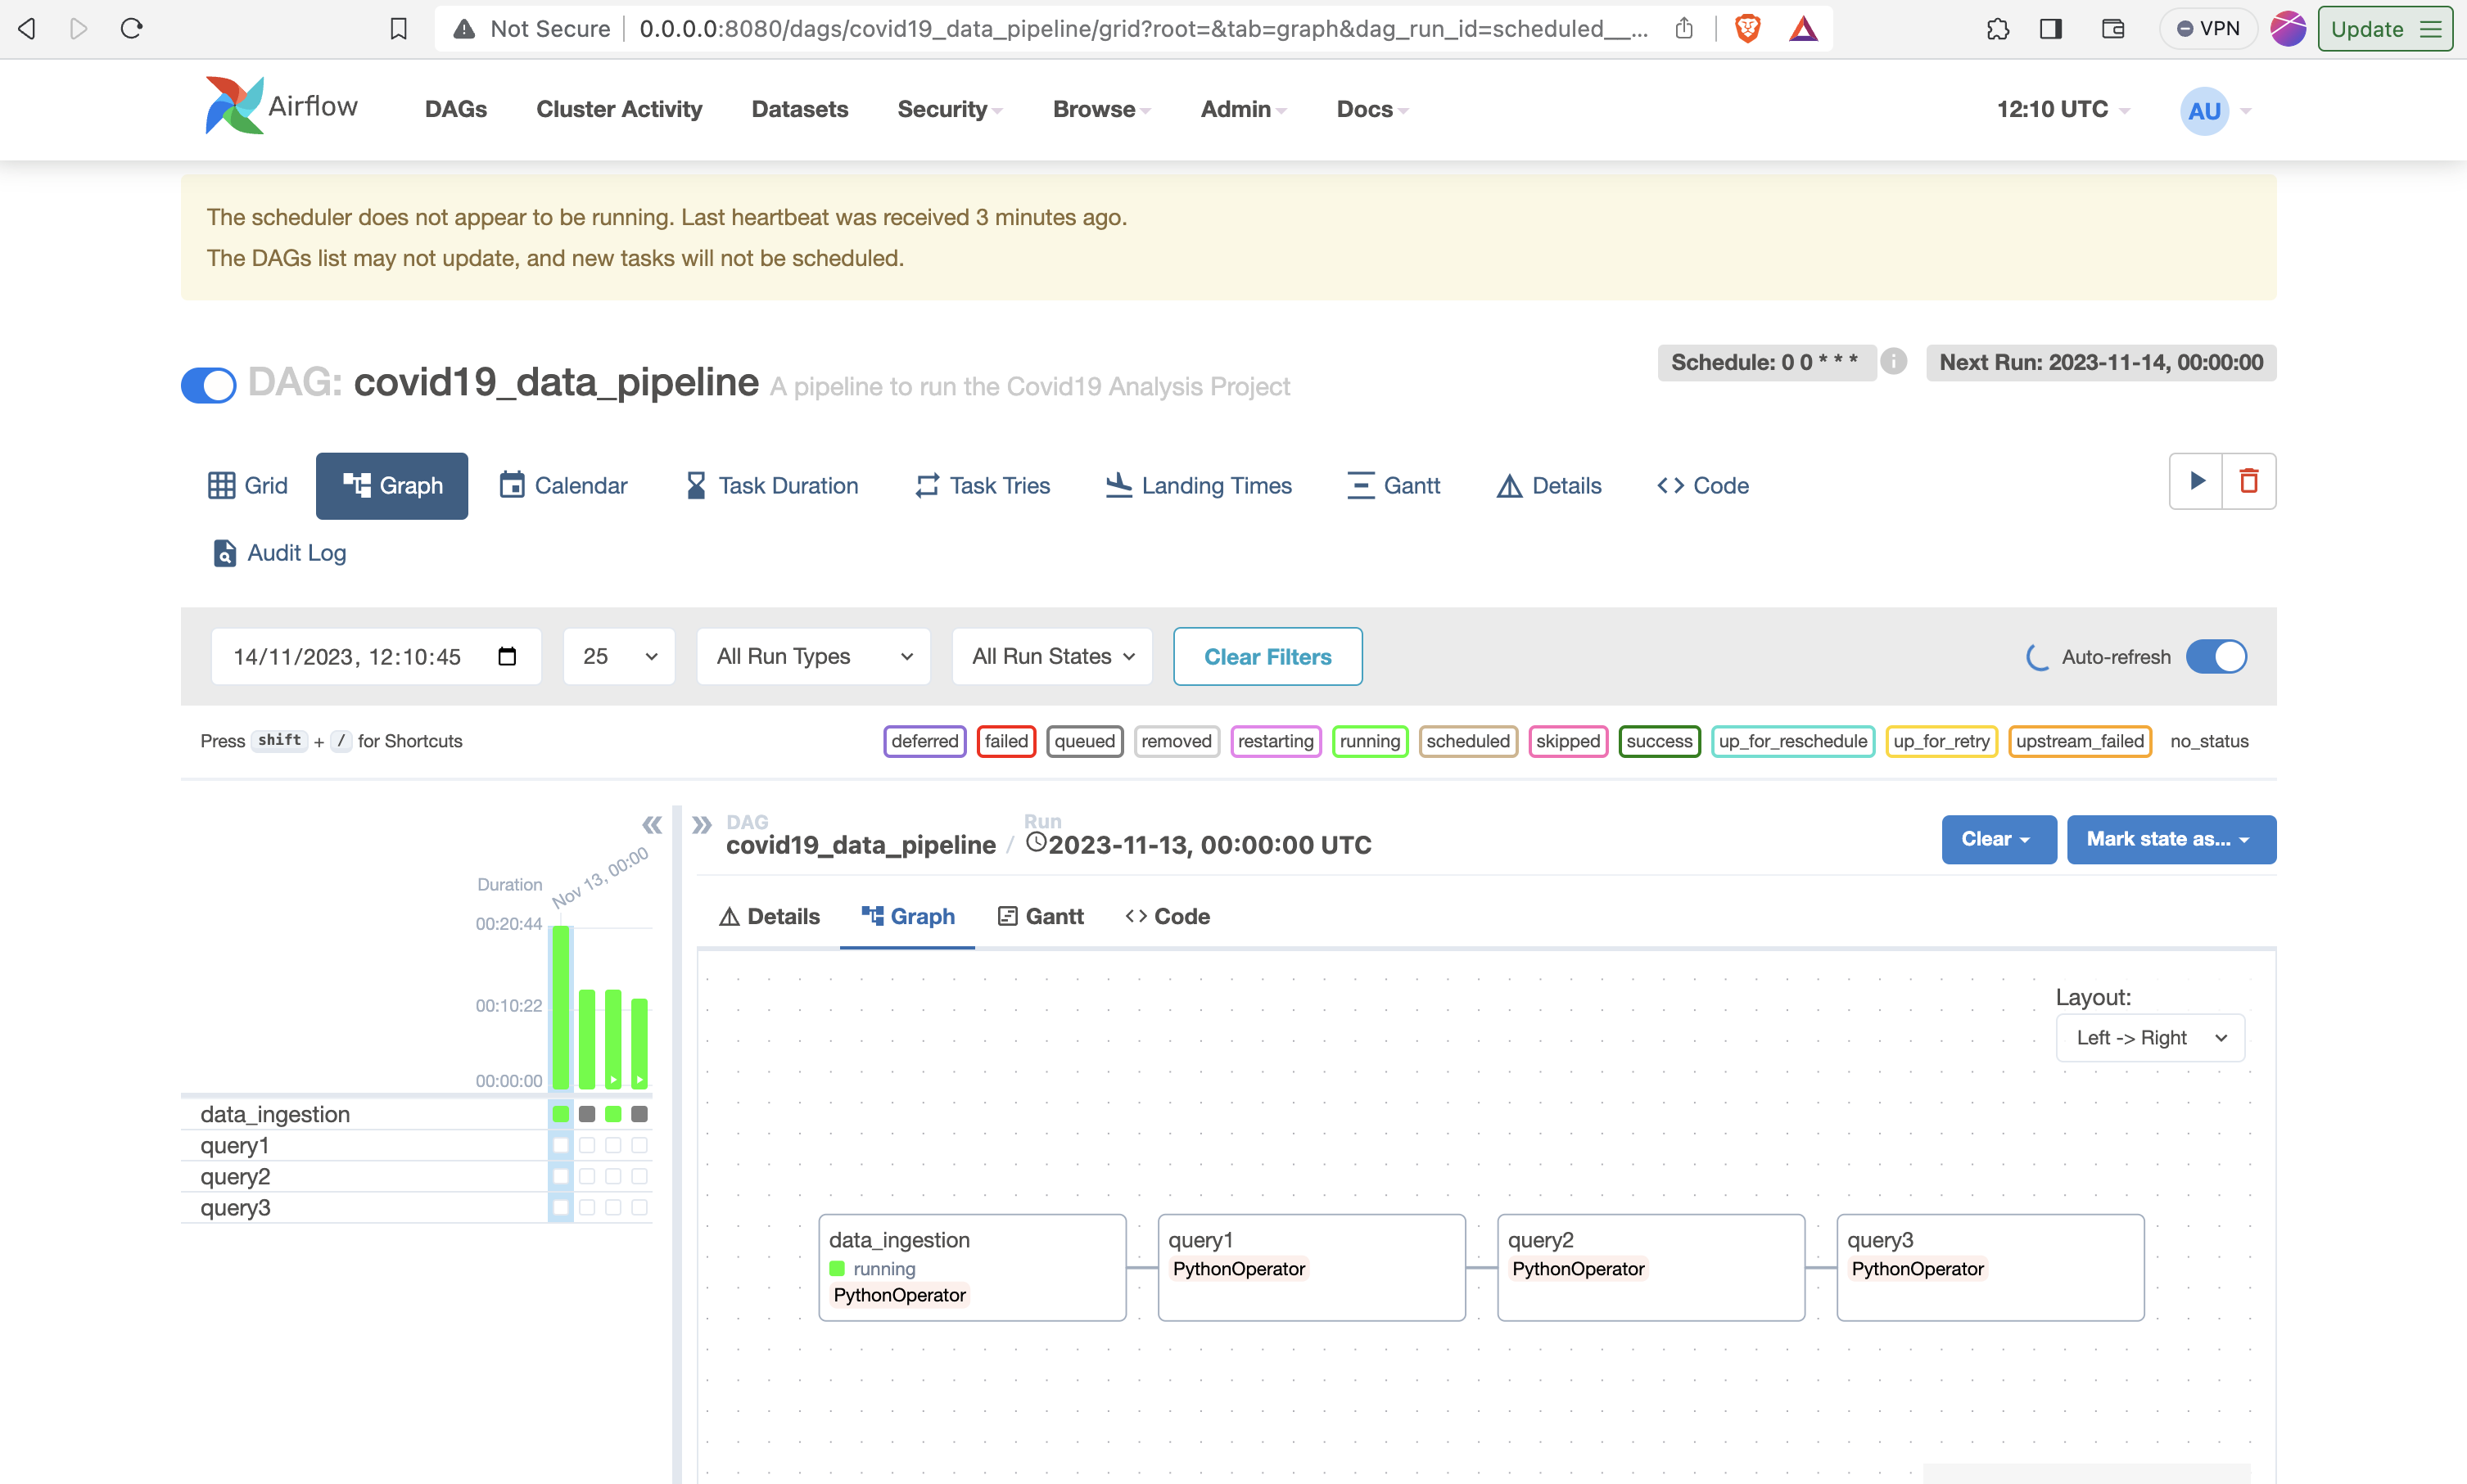
\includegraphics[width=1\linewidth]{images/Screenshot 2023-11-14 at 12.10.48.png}
    \caption{Apache Airflow DAG Graph}\label{fig:apache-airflow}
\end{figure}

\newpage
\chapter{Results \& Discussion}

\section{Queries Results}
The programme was last run on 18 November 2023. The appendix~\ref{appendix:4}
shows the output of the program on the terminal.

\subsection{Query 1}

The first query takes around 3 seconds, and the table
~\ref{tab:query1-results-sample} shows a sample of the data calculated during
the task. In order to evaluate performance, an equivalent script not using
Spark was run. Execution time was 0.5 sec. The~\ref{sec:discussion-of-results}
section will cover this point. The results are consistent with what was
expected~\cite{NYT}. For example, the figure~\ref{fig:sub1} shows that Brazil
was heavily impacted by the pandemic, reaching an average peak in February
2022. The same is true for Korea in figure~\ref{fig:sub2} and the United States
in figure~\ref{fig:sub3}, which were heavily impacted.

\begin{table}[h]
    \centering
    \captionsetup{font=large}
    \caption{Query 1 Results Sample}
    \normalsize
    \begin{tabular}{|l|c|c|c|c|c|}
        \hline
          & Country/Region & Year & Month & Average            \\
        \hline
        1 & Afghanistan    & 2020 & 1     & 0.0                \\
        2 & Afghanistan    & 2020 & 2     & 0.1724137931034483 \\
        3 & Afghanistan    & 2020 & 3     & 5.193548387096774  \\
        4 & Afghanistan    & 2020 & 4     & 55.36666666666667  \\
        5 & Afghanistan    & 2020 & 5     & 430.741935483871   \\
        \hline
    \end{tabular}\label{tab:query1-results-sample}
\end{table}

\begin{figure}[H]
    \vspace{-15pt}
    \centering
    \begin{subfigure}[b]{\linewidth}
        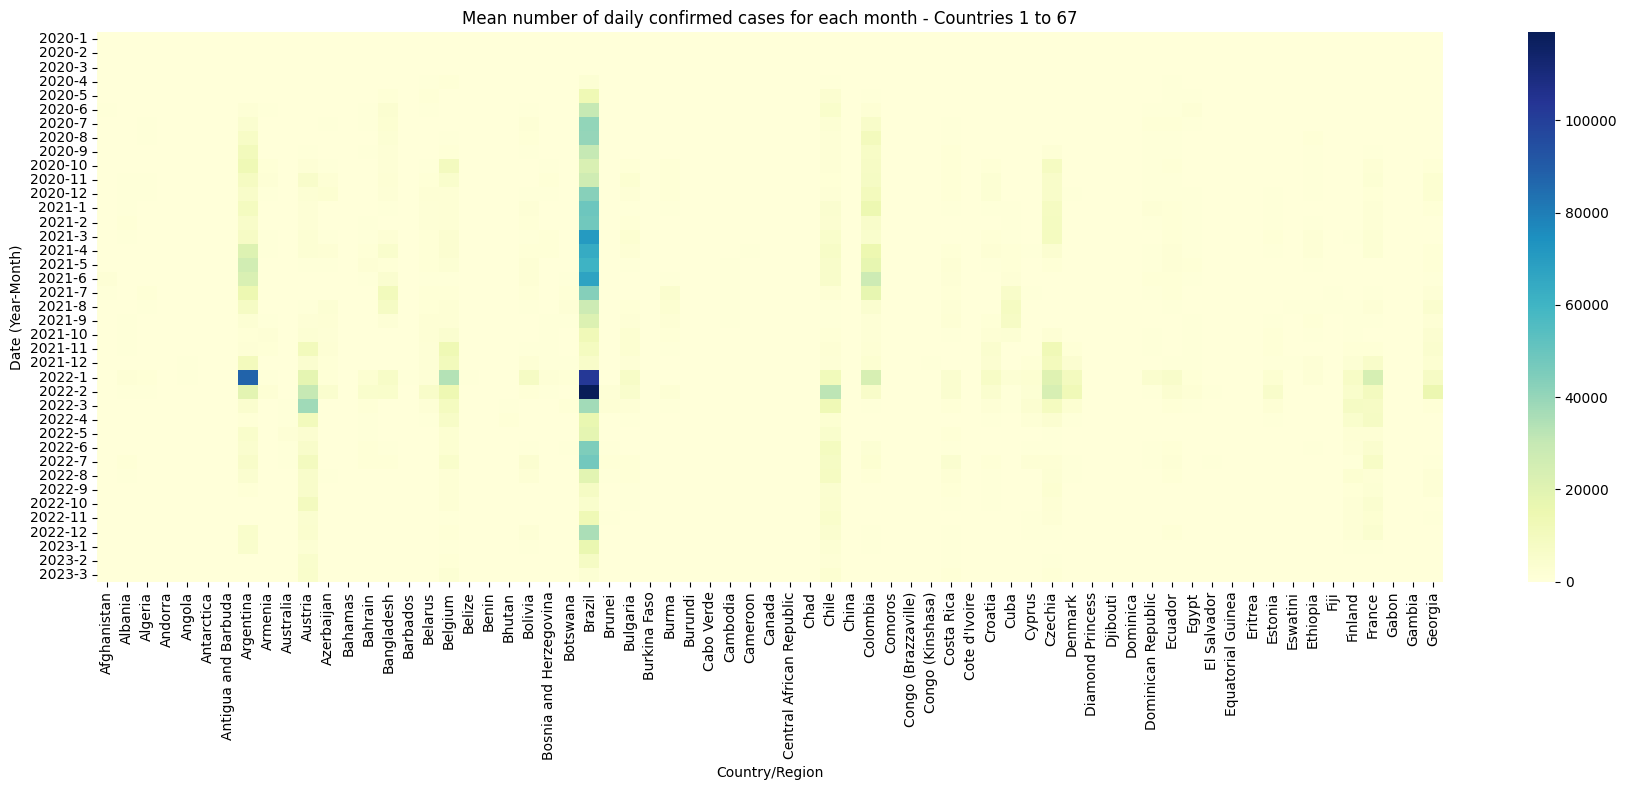
\includegraphics[width=\linewidth]{images/mean-daily-confirmed-cases-per-month-1.png}
        \caption{Countries 1 to 67}\label{fig:sub1}
        \vspace{-2pt}
    \end{subfigure}
    \hfill
    \begin{subfigure}[b]{\linewidth}
        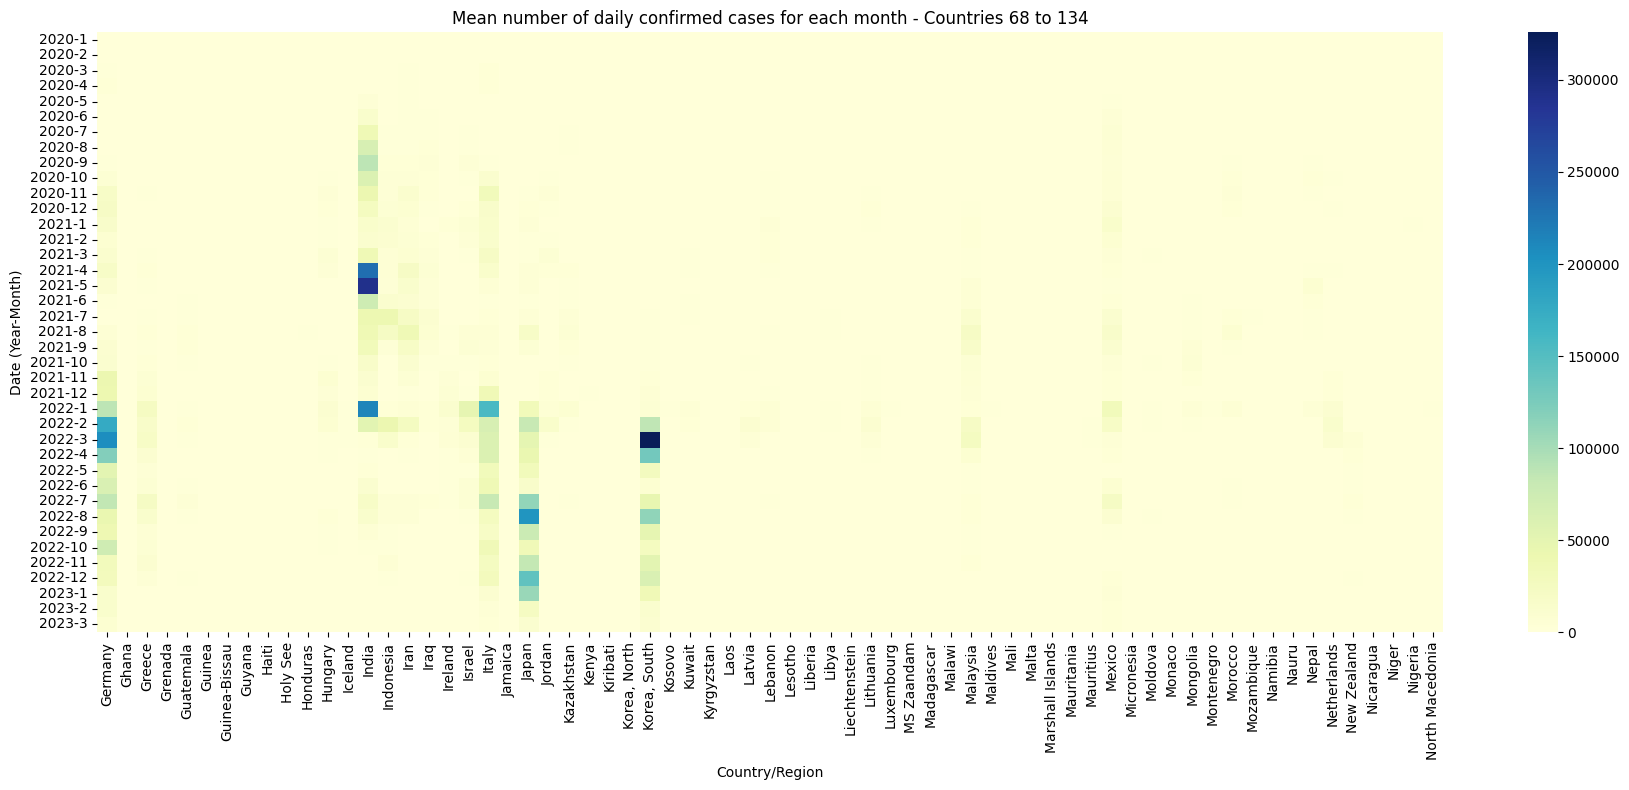
\includegraphics[width=\linewidth]{images/mean-daily-confirmed-cases-per-month-2.png}
        \caption{Countries 68 to 134}\label{fig:sub2}
        \vspace{-2pt}
    \end{subfigure}
    \hfill
    \begin{subfigure}[b]{\linewidth}
        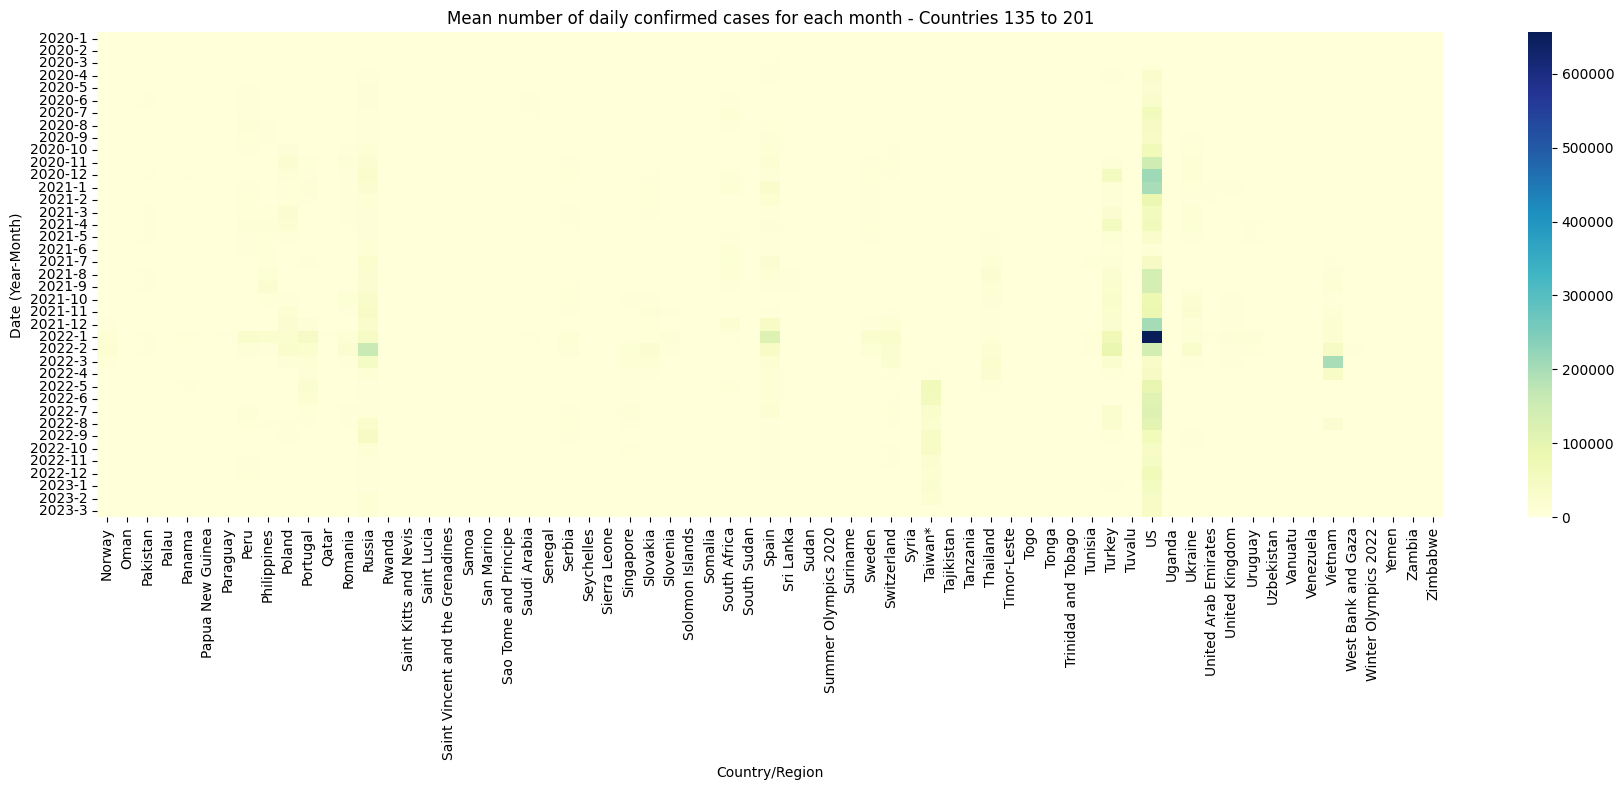
\includegraphics[width=\linewidth]{images/mean-daily-confirmed-cases-per-month-3.png}
        \caption{Countries 135 to 201}\label{fig:sub3}
        \vspace{-5pt}
    \end{subfigure}
    \caption{Mean Daily Confirmed Cases Per Month}\label{fig:mean-daily-confirmed-cases-per-month}
\end{figure}

\newpage
\subsection{Query 2}

The second query takes around 15 seconds, and the
table~\ref{tab:query2-results-sample} shows a sample of the data calculated
during the task. In order to evaluate performance, an equivalent script not
using Spark was run. Execution time was 6 sec.
The~\ref{sec:discussion-of-results} section will cover this point. Locations
used to compute the statistics are shown on the map of
figure~\ref{fig:top-100-locations-most-affected}. The area of the circles is
proportional to how the location has been affected by the pandemic.

\begin{figure}[H]
    \centering
    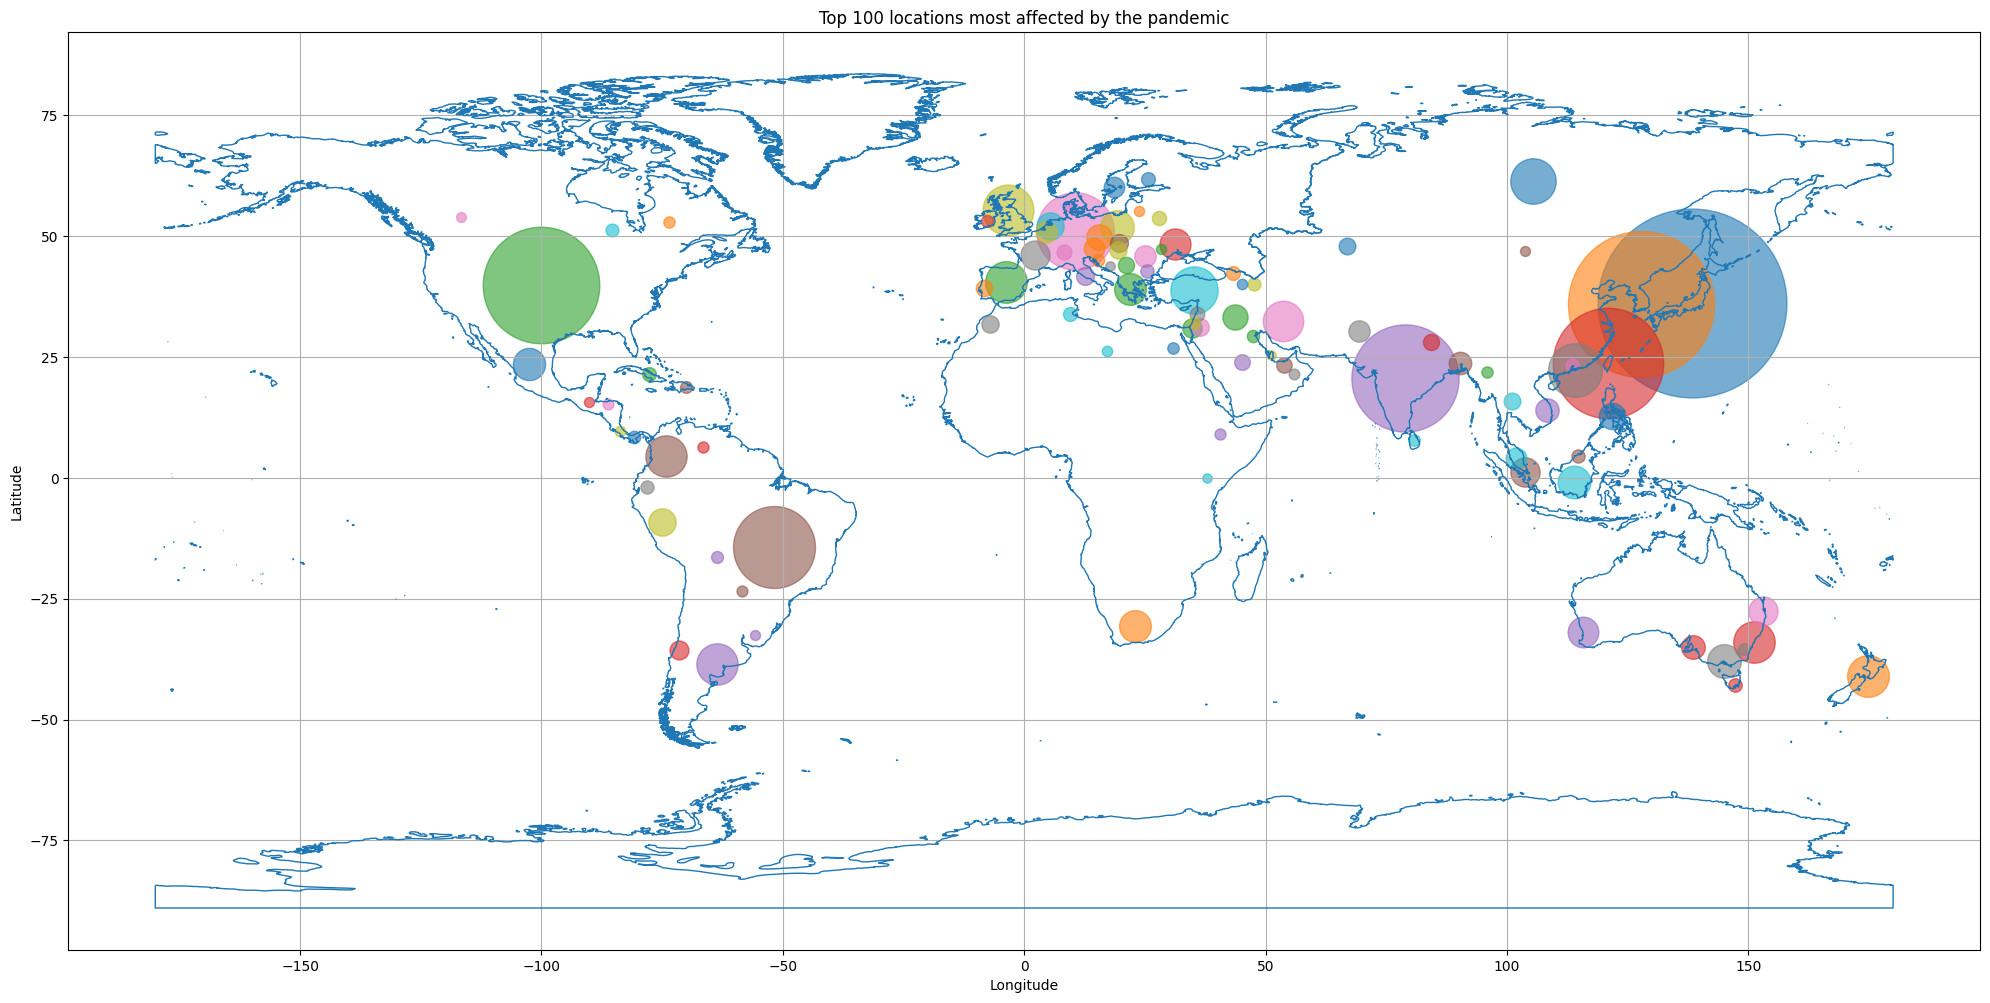
\includegraphics[width=1\linewidth]{images/top-100-locations-most-affected.png}
    \caption{Top 100 Locations most affected by the pandemic}\label{fig:top-100-locations-most-affected}
\end{figure}

\begin{table}[H]
    \centering
    \captionsetup{font=large}
    \caption{Query 2 Results Sample}
    \normalsize
    \begin{tabular}{|l|c|c|c|c|c|c|c|}
        \hline
           & Continent & WeekRange             & Mean     & Std      & Min & Max \\
        \hline
        1  & Africa    & 19/01/2020-25/01/2020 & 0.0      & 0.0      & 0   & 0   \\
        2  & Africa    & 26/01/2020-01/02/2020 & 0.0      & 0.0      & 0   & 0   \\
        3  & Africa    & 02/02/2020-08/02/2020 & 0.0      & 0.0      & 0   & 0   \\
        4  & Africa    & 09/02/2020-15/02/2020 & 0.0      & 0.0      & 0   & 0   \\
        5  & Africa    & 16/02/2020-22/02/2020 & 0.0      & 0.0      & 0   & 0   \\
        6  & Africa    & 23/02/2020-29/02/2020 & 0.0      & 0.0      & 0   & 0   \\
        7  & Africa    & 01/03/2020-07/03/2020 & 0.02857  & 0.16903  & 0   & 1   \\
        8  & Africa    & 08/03/2020-14/03/2020 & 0.65714  & 1.73108  & 0   & 9   \\
        9  & Africa    & 15/03/2020-21/03/2020 & 2.74285  & 4.53964  & 0   & 17  \\
        10 & Africa    & 22/03/2020-28/03/2020 & 12.62857 & 15.33754 & 0   & 59  \\
        11 & Africa    & 29/03/2020-04/04/2020 & 14.97142 & 19.31242 & 0   & 82  \\
        \hline
    \end{tabular}\label{tab:query2-results-sample}
\end{table}

\newpage

The figures below~\ref{fig:mean-confirmed-cases-by-week-and-continent}
and~\ref{fig:std-confirmed-cases-by-week-and-continent} show the mean and
standard deviation of the number of confirmed cases by week and continent. The
results are consistent with expectations: the continents most affected are
America and Europe~\cite{NYT}.

\begin{figure}[H]
    \centering
    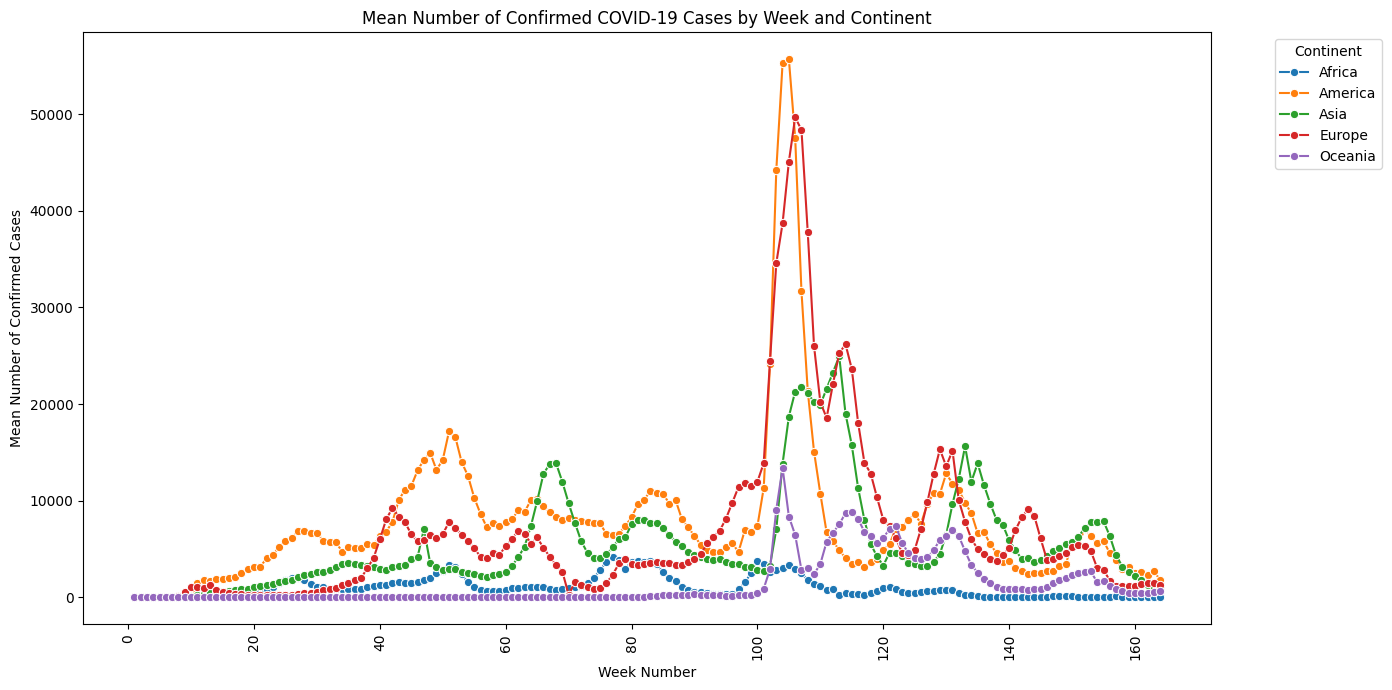
\includegraphics[width=1\textwidth]{images/mean-confirmed-cases-by-week-and-continent.png}
    \caption{Mean Confimed Cases By Week and Continent}\label{fig:mean-confirmed-cases-by-week-and-continent}
\end{figure}

\begin{figure}[H]
    \centering
    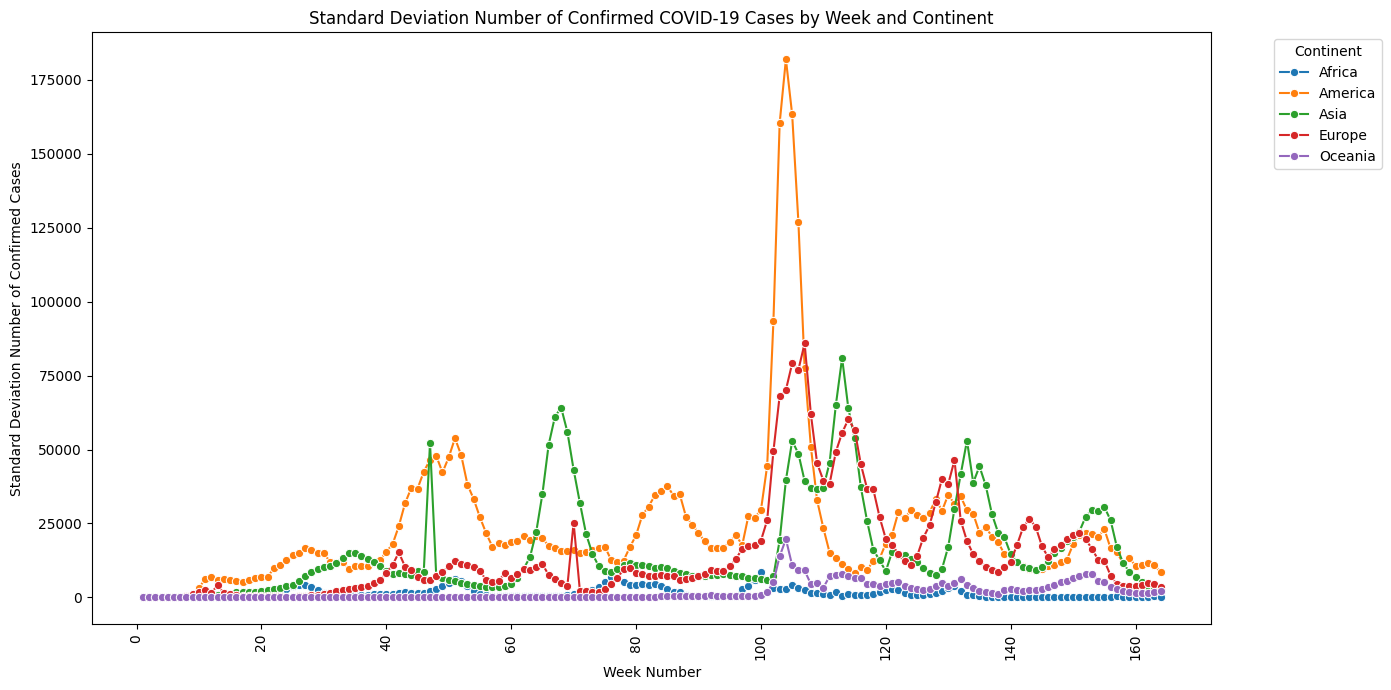
\includegraphics[width=1\textwidth]{images/std-confirmed-cases-by-week-and-continent.png}
    \caption{Standard Deviation Confimed Cases By Week and Continent}\label{fig:std-confirmed-cases-by-week-and-continent}
\end{figure}

\newpage
The figures~\ref{fig:max-confirmed-cases-by-week-and-continent} and~\ref{fig:min-confirmed-cases-by-week-and-continent} show the maximum and minimum of the number of confirmed cases by week and continent.

\begin{figure}[H]
    \centering
    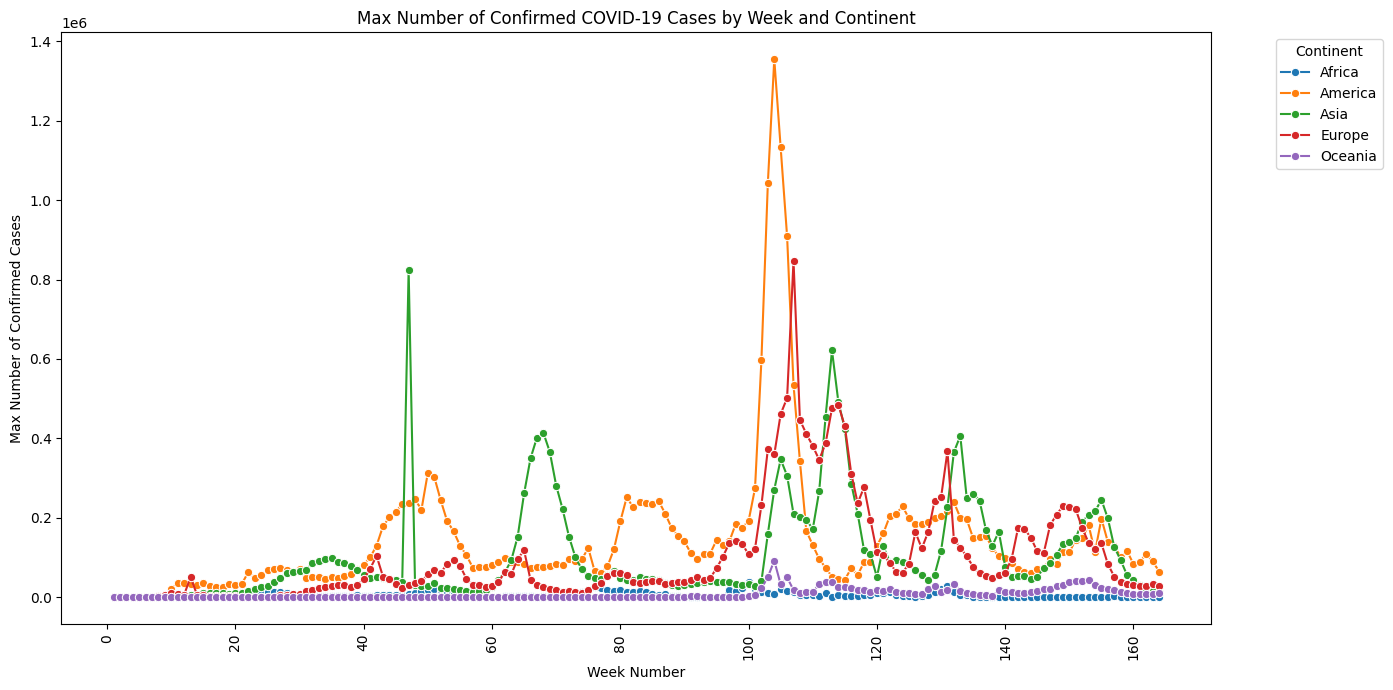
\includegraphics[width=1\textwidth]{images/max-confirmed-cases-by-week-and-continent.png}
    \caption{Maximum Confimed Cases By Week and Continent}\label{fig:max-confirmed-cases-by-week-and-continent}
\end{figure}

\begin{figure}[H]
    \centering
    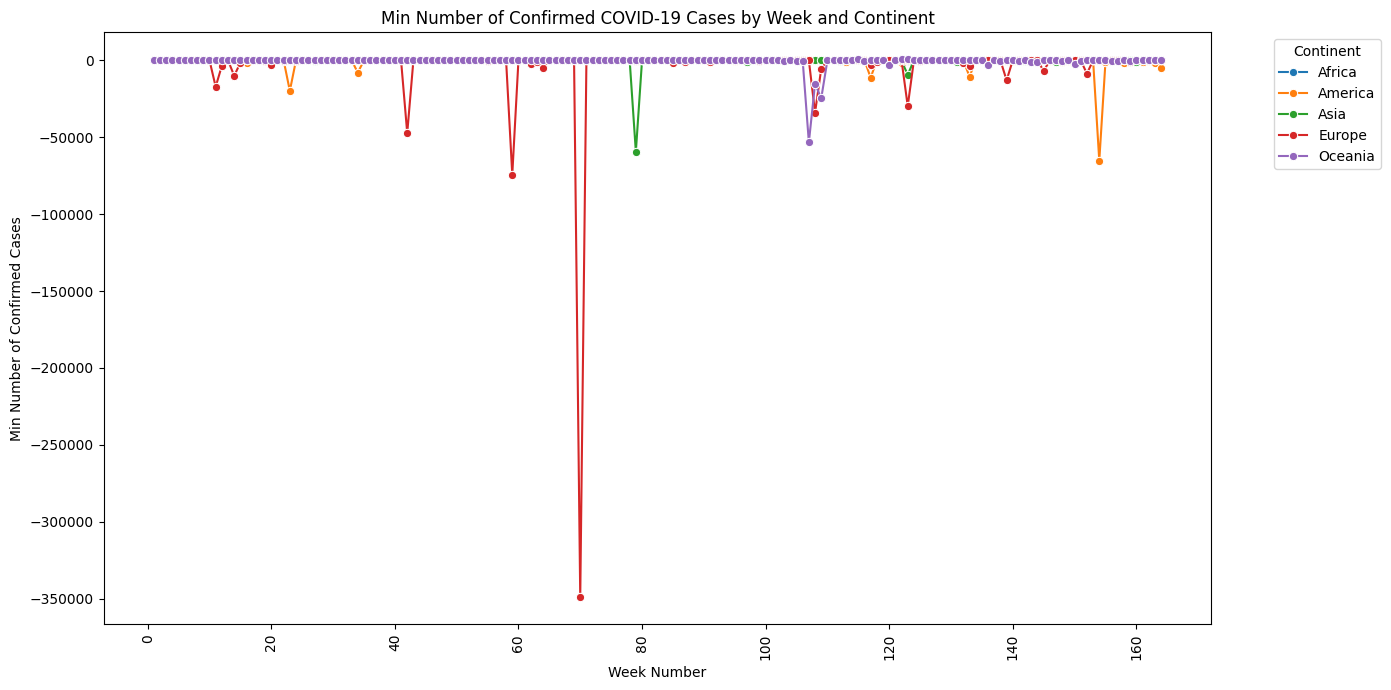
\includegraphics[width=1\textwidth]{images/min-confirmed-cases-by-week-and-continent.png}
    \caption{Minimum Confimed Cases By Week and Continent}\label{fig:min-confirmed-cases-by-week-and-continent}
\end{figure}

\newpage
\subsection{Query 3}

The third query takes around 3 minutes as clustering with the custom
implementation takes 60 seconds and clustering with the Spark MLlib
implementation takes 110 seconds. The
table~\ref{tab:query3-custom-results-sample} shows a sample of the data
calculated during the task with the custom implementation and the
table~\ref{tab:query3-spark-results-sample} with the Spark MLlib
implementation. Locations used to compute the statistics are shown on the map
of figure~\ref{fig:top-50-locations-most-affected}. The area of the circles is
proportional to how the location has been affected by the pandemic.

\begin{figure}[H]
    \centering
    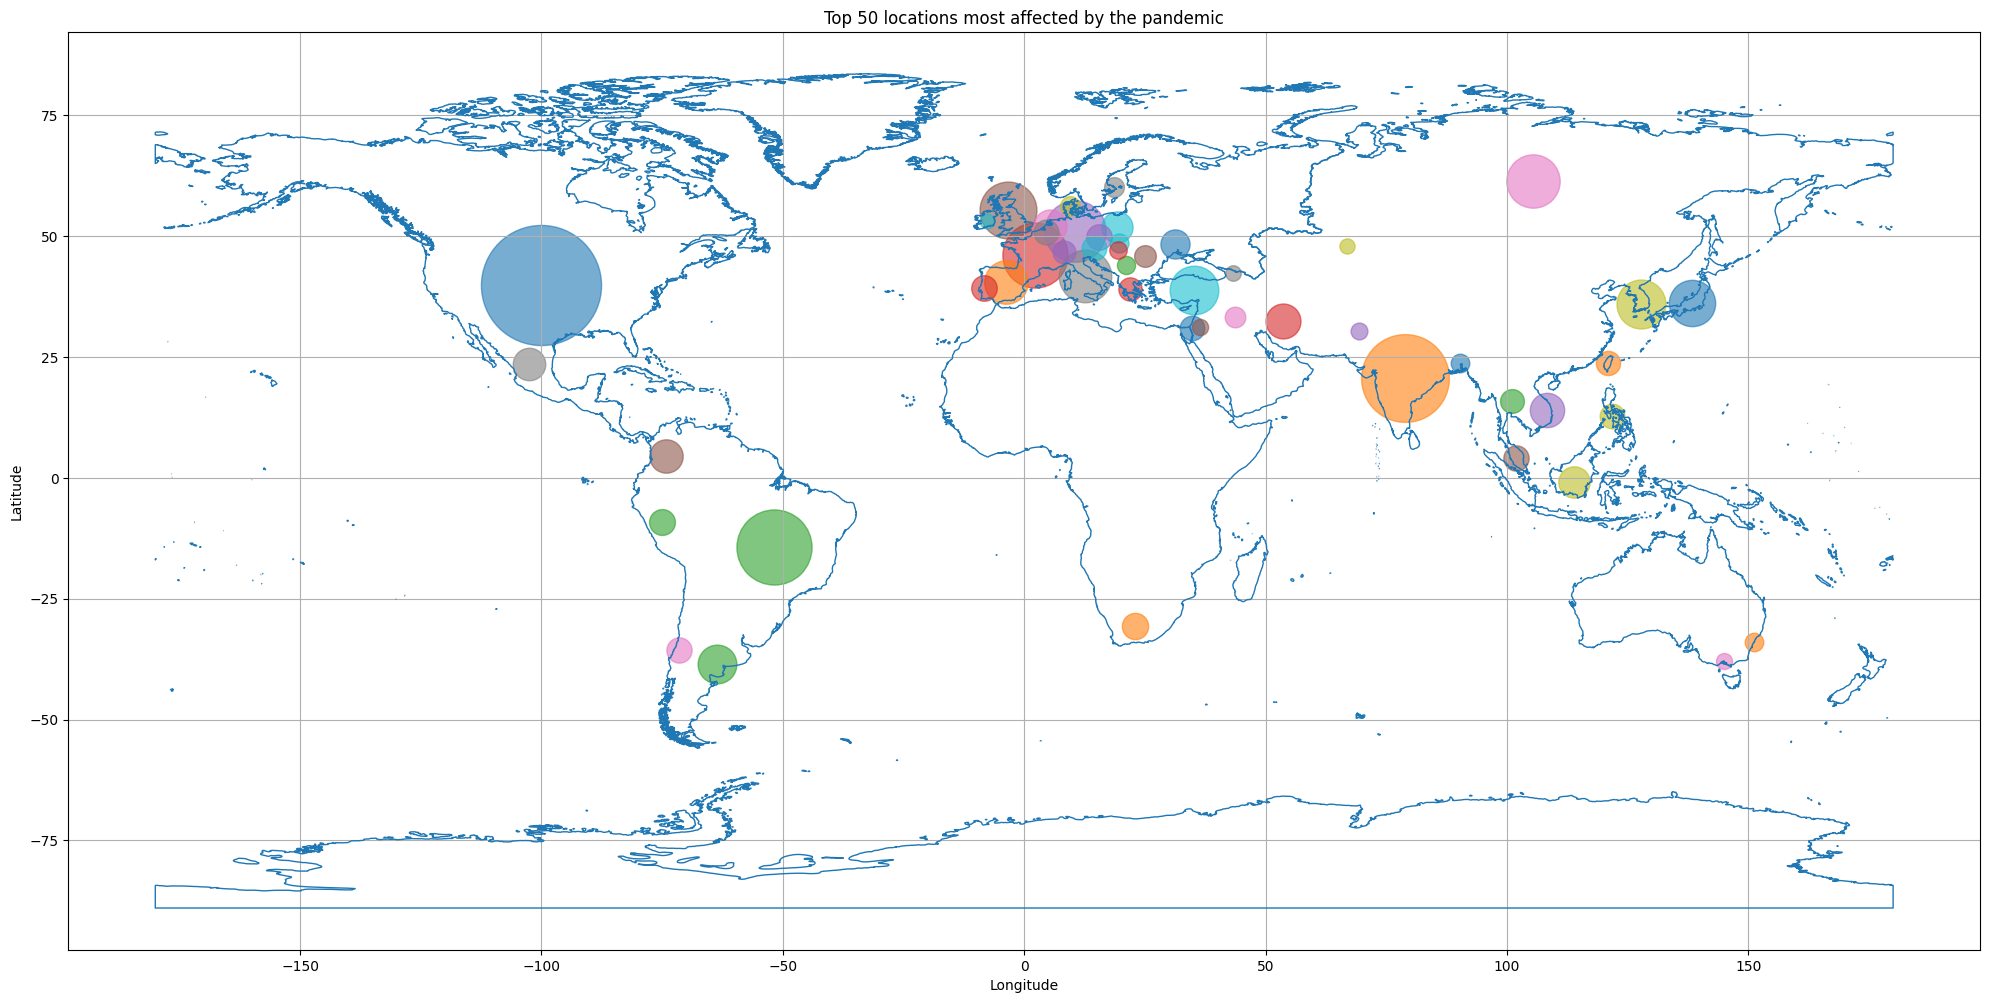
\includegraphics[width=1\linewidth]{images/top-50-locations-most-affected.png}
    \caption{Top 50 Locations most affected by the pandemic}\label{fig:top-50-locations-most-affected}
\end{figure}

\begin{table}[H]
    \centering
    \captionsetup{font=large}
    \caption{Query 3 Results Sample - Custom KMeans Clustering}
    \normalsize
    \begin{tabular}{|l|c|c|c|c|}
        \hline
          & Location  & Month   & Cluster \\
        \hline
        1 & Argentina & 2020-01 & 2       \\
        2 & Austria   & 2020-01 & 2       \\
        3 & Brazil    & 2020-01 & 2       \\
        4 & Czechia   & 2020-01 & 2       \\
        5 & France    & 2020-01 & 1       \\
        \hline
    \end{tabular}\label{tab:query3-custom-results-sample}
\end{table}

\begin{table}[H]
    \centering
    \captionsetup{font=large}
    \caption{Query 3 Results Sample - Spark MLlib KMeans Clustering}
    \normalsize
    \begin{tabular}{|l|c|c|c|c|}
        \hline
          & Location  & Month   & Cluster \\
        \hline
        1 & Argentina & 2020-01 & 2       \\
        2 & Austria   & 2020-01 & 0       \\
        3 & Brazil    & 2020-01 & 2       \\
        4 & Czechia   & 2020-01 & 2       \\
        5 & France    & 2020-01 & 1       \\
        \hline
    \end{tabular}\label{tab:query3-spark-results-sample}
\end{table}

\newpage

The figures below~\ref{fig:covid-19-clusters-custom}
and~\ref{fig:covid-19-clusters-spark} show the clusters of the top 50 locations
most affected by the pandemic in March 2020. The clusters are represented by
different colours.

\begin{figure}[H]
    \centering
    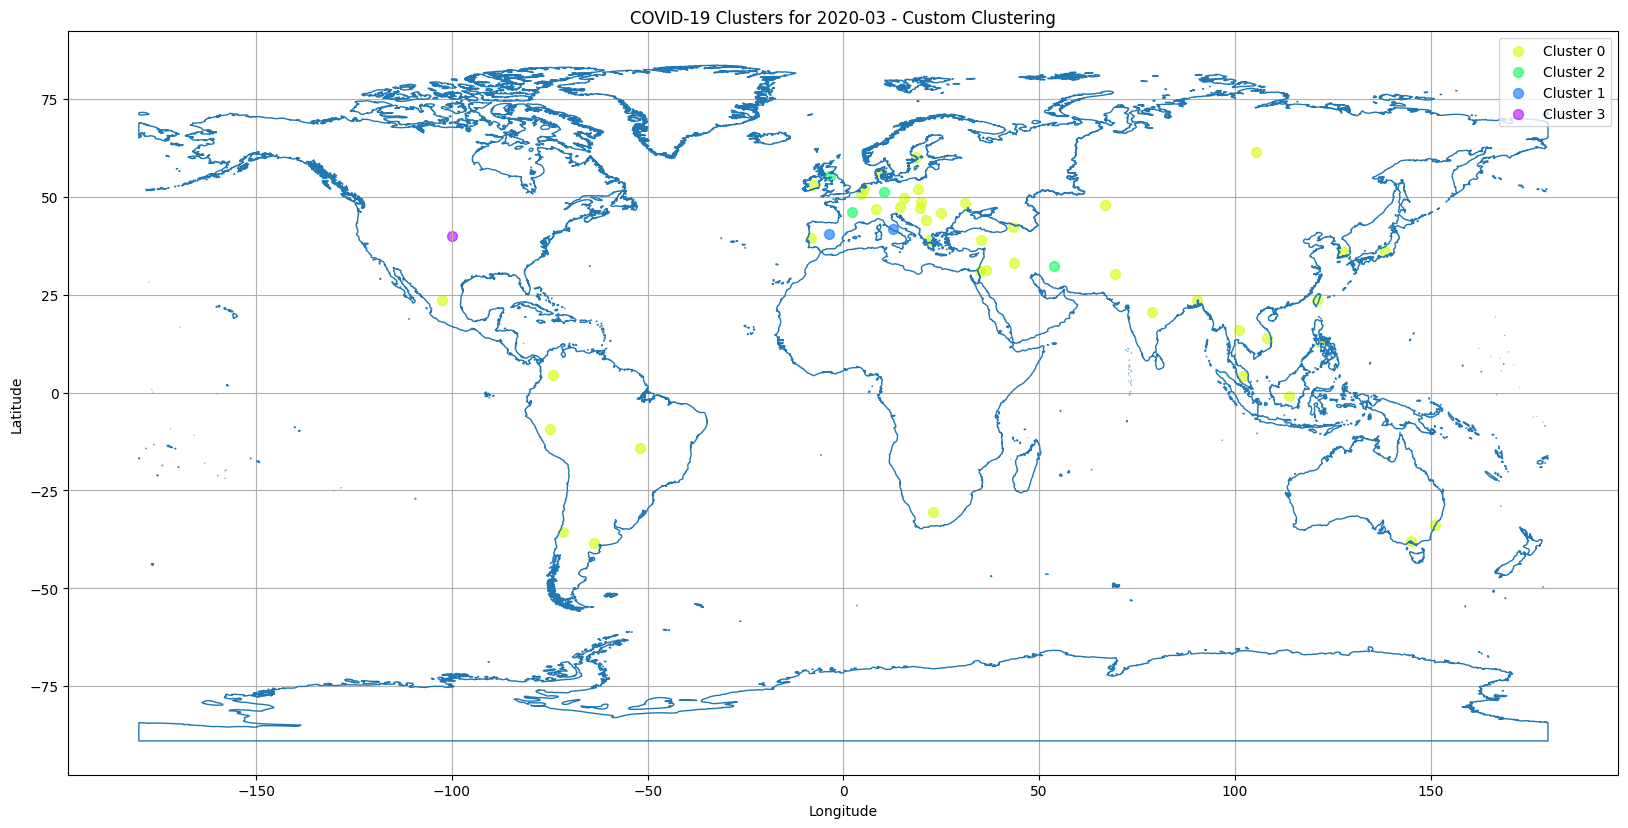
\includegraphics[width=1\textwidth]{images/covid-19-clusters-custom.png}
    \caption{Custom KMeans Clustering on 03/2020}\label{fig:covid-19-clusters-custom}
\end{figure}

\begin{figure}[H]
    \centering
    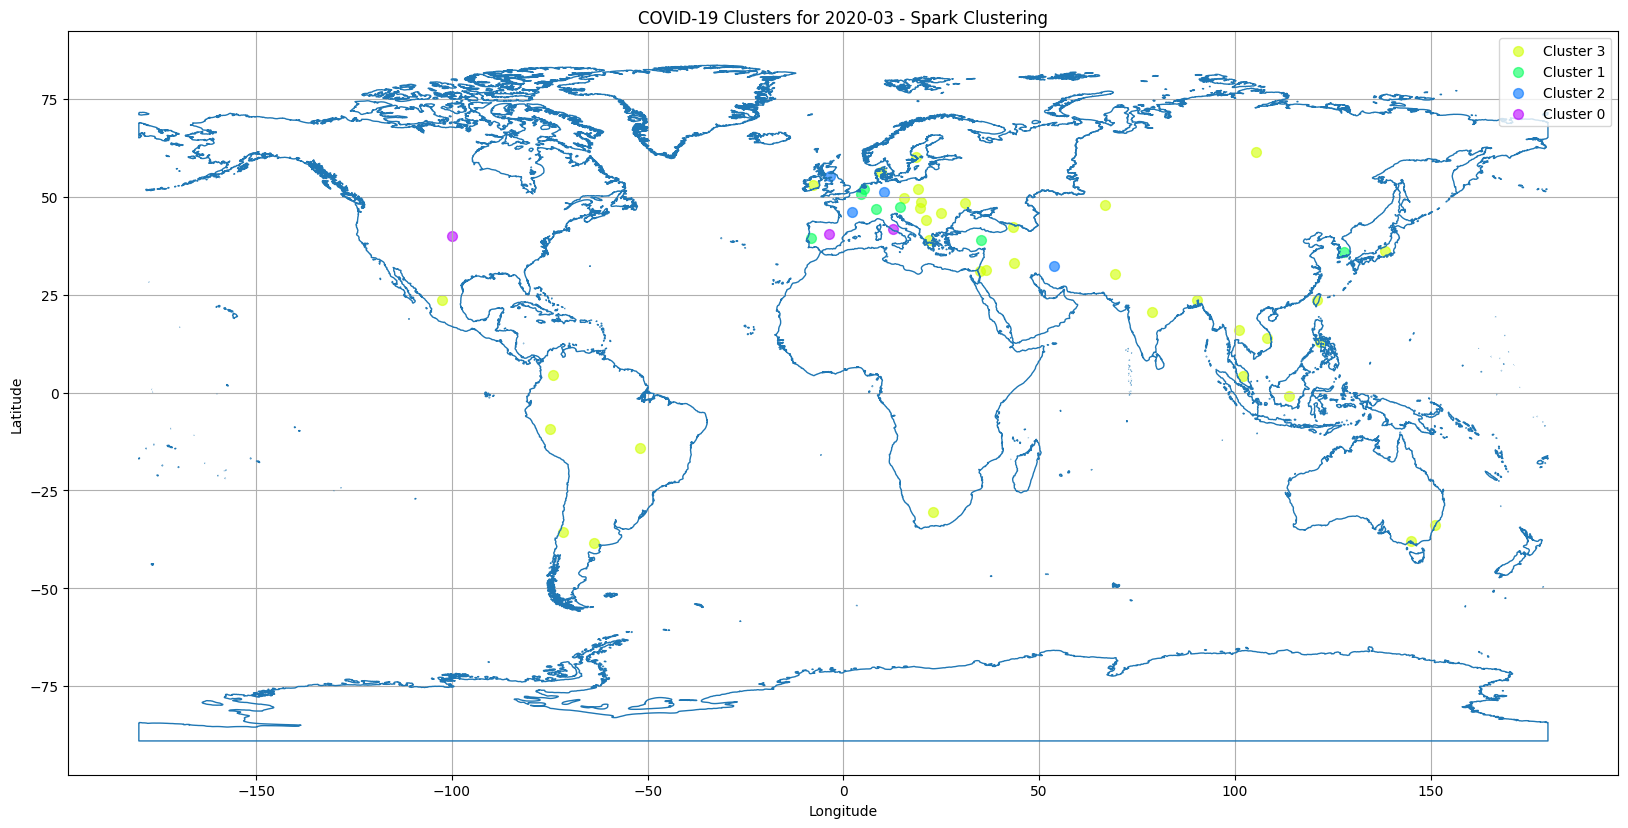
\includegraphics[width=1\textwidth]{images/covid-19-clusters-spark.png}
    \caption{Spark MLlib KMeans Clustering on 03/2020}\label{fig:covid-19-clusters-spark}
\end{figure}

\newpage

\section{Discussion of Results}\label{sec:discussion-of-results}
As the previous results show, it seems that scripts not using Spark are faster.
While these differences in execution time may seem surprising at first glance,
they can in fact be attributed to several factors:

\begin{enumerate}
    \item \textbf{Data size and structure:} The DataFrame, with its 289 entries and 1147 columns occupying 2.5 MB of memory, is relatively modest in size. Pandas is particularly efficient at processing such large amounts of data in memory on a single node. Spark, on the other hand, is designed for distributed processing of large datasets. In this case, the overheads of distributing the data and managing the Spark environment may outweigh the benefits of using it for smaller datasets.
    \item \textbf{Operational efficiency:} Pandas performs vectorised operations that are optimised for speed, especially with datasets that fit easily into memory on a single computer. Spark, while powerful for processing large volumes of data, introduces an initial overhead for distributing data and configuring the distributed environment, which can slow down processing for smaller datasets.
    \item \textbf{Complexity of the environment:} Complexity of the environment: Running operations in a Spark environment involves initializing a cluster (even in local mode), distributing tasks, and managing distributed memory, which adds extra processing time compared to running in-memory Pandas directly.
\end{enumerate}

Thus in this project run locally, Pandas is faster than Spark, due to its
efficient management of in-memory operations on a single node. Spark's
distributed processing overhead makes it less efficient for such tasks.

\newpage
\section{Ethical Considerations and Challenges}

\newpage
\chapter{Conclusion}

\bibliographystyle{CranfieldNumbered}
\bibliography{CUCitations}

\appendix
\begin{appendices}
    \chapter{Documentation}
    \begin{subappendices}
        \section{Project tree}
        \begin{lstlisting}[breaklines=true, basicstyle=\small]
        lib/
        collecting.py
        processing.py
        storing.py
        scripts/
            get_iam_credentials.sh
            start_spark_job.sh
        services/
            get_iam_credentials.service
            spark_python_job.service
            grafana_server.service
        artillery_load_test.yml
        ingestion_iot_data_flatten.py
        main.py
        README.md
        requirements.txt
        \end{lstlisting}

        \section{Getting Started}
        To run the program, follow these steps:
        \begin{enumerate}
            \itemindent=17.87pt
            \item Create a virtual environment using \texttt{python3 -m venv venv}.
            \item Activate the virtual environment using \texttt{source venv/bin/activate}.
            \item Install the required dependencies using \texttt{pip3 install -r
                      requirements.txt}.
            \item Run the program using \texttt{python3 main.py}.
            \item Visualise the results using \texttt{visualisation.ipynb} (Jupyter Notebook).
        \end{enumerate}

        \section{Detailed Features of Functions}
        \begin{description}
            \item \texttt{collecting.py}
                  \begin{itemize}
                      \item \texttt{fetch\_sensors\_data(sparkSession)}: Function to ingest the latest data from the sensors and returns it as a Spark DataFrame.
                  \end{itemize}

            \item \texttt{processing.py}
                  \begin{itemize}
                      \item \texttt{get\_aqi\_value\_p25(value)}: Function for calculating the AQI value for PM2.5.
                      \item \texttt{get\_aqi\_value\_p10(value)}: Function for calculating the AQI value for PM10.
                      \item \texttt{computeAQI(df)}: Function for calculating the AQI value for each particulate matter sensor and returning the DataFrame with the AQI column.
                  \end{itemize}

            \item \texttt{storing.py}
                  \begin{itemize}
                      \item \texttt{keepOnlyUpdatedRows(database\_name, table\_name, df)}: Function for keeping only the rows that have been updated in the DataFrame.
                      \item \texttt{\_print\_rejected\_records\_exceptions(err)}: Internal function for printing the rejected records exceptions.
                      \item \texttt{write\_records(database\_name, table\_name, client, records)}: Internal function for writing a batch of records to the Timestream database.
                      \item \texttt{writeToTimestream(database\_name, table\_name, partionned\_df)}: Function for writing the DataFrame to the Timestream database.
                  \end{itemize}
        \end{description}
    \end{subappendices}

    \chapter{Source Codes}
    \begin{subappendices}
        \section{Ingestion, Processing \& Storing Pipeline Source Code}
        \lstset{style=python}
        \lstinputlisting[style=mystyle]{../main.py}

        \section{Data Collecting Source Code}
        \lstset{style=python}
        \lstinputlisting[style=mystyle]{../lib/collecting.py}

        \section{Data Processing Source Code}
        \lstset{style=python}
        \lstinputlisting[style=mystyle]{../lib/processing.py}

        \section{Data Storing Source Code}
        \lstset{style=python}
        \lstinputlisting[style=mystyle]{../lib/storing.py}

        \section { Scripts \& Services Source Code }
        \subsection{Scripts}

        Script used by the \texttt{get\_iam\_credentials} service to retrieve the IAM
        credentials from the metadata server. \lstset{style=terminal}
        \lstinputlisting[style=mystyle]{../scripts/get_iam_credentials.sh}

        Script used by the \texttt{spark\_python\_job} service to run the Python Spark
        job. \lstset{style=terminal}
        \lstinputlisting[style=mystyle]{../scripts/start_spark_job.sh}

        \subsection{Services}

        Service used by the Ubuntu EC2 instance to retrieve the IAM credentials from
        the metadata server. \lstset{style=terminal}
        \lstinputlisting[style=mystyle]{../services/get_iam_credentials.service}

        Service used by the Ubuntu EC2 instance to run the Python Spark job (Data
        Collecting, Processing and Storing). \lstset{style=terminal}
        \lstinputlisting[style=mystyle]{../services/spark_python_job.service}

        Service used by the Linux EC2 instances to run the Grafana server (Data
        Distributing). \lstset{style=terminal}
        \lstinputlisting[style=mystyle]{../services/grafana_server.service}
    \end{subappendices}
\end{appendices}

\end{document}

\section{Scripts \& Services}
\begin{subappendices}

